\documentclass[a4paper]{article}

\usepackage[english]{babel}
\usepackage[utf8]{inputenc}
\usepackage{amsmath}
\usepackage{graphicx}
\usepackage{minted}
\usepackage{algorithm}
\usepackage[noend]{algpseudocode}
\usepackage[colorinlistoftodos]{todonotes}
\usepackage{multirow}
\usepackage{parskip}

% empty set package
\usepackage{amssymb}

% Automata package
\usepackage{pgf,tikz}
\usetikzlibrary{shapes,arrows,automata}


\title{CSCE 828 - Homework 4}
\author{Tian Gao}
\begin{document}
\maketitle


% Question 1
1.\\
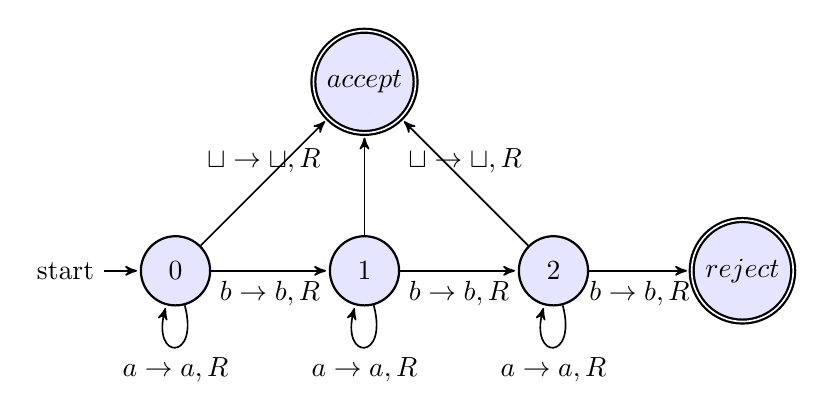
\begin{tikzpicture}[->,>=stealth',shorten >=1pt,auto,node distance=2.4cm,on grid,semithick, every state/.style={fill=blue!10,thick}]
\node[initial,state] 	 (0)              {$0$};
\node[state]        	 (1) [right of=0] {$1$};
\node[state]        	 (2) [right of=1] {$2$};
\node[state,accepting]   (r) [right of=2] {$reject$};
\node[state,accepting]	 (a) [above of=1] {$accept$};

\path[->] 
	(0) edge [below]        node {$ b \rightarrow b,R $} (1)
    (0) edge [loop below]   node {$ a \rightarrow a,R $} (0)
	(1) edge [below]        node {$ b \rightarrow b,R $} (2)
    (1) edge [loop below]   node {$ a \rightarrow a,R $} (1)
	(2) edge [below] 		node {$ b \rightarrow b,R $} (r)
	(2) edge [loop below] 	node {$ a \rightarrow a,R $} (2)  
	(0) edge [above]        node {$ \sqcup \rightarrow \sqcup,R $} (a)    
    (1) edge [above]        node {$$} (a)
    (2) edge [above]        node {$ \sqcup \rightarrow \sqcup,R $} (a)
    
;    
\end{tikzpicture}\\

% Question 2
2.\\
step1: prove that standard TM can simulate 2-PDA.\\
2-PDA can be simulated by 2-tape non-deterministic TM and 2-tape non-deterministic TM can be simulated by standard TM.\\
So standard TM can simulate 2-PDA.\\
\\
step2: prove that 2-PDA can simulate standard TM.\\
Let T be a TM, T = $(Q_T, \Sigma_T, \Gamma_T, \delta_T, q_{0,T}, q_{accept}, q_{reject})$\\
Let M be a 2-PDA, M = $(Q_M, \Sigma_M, \Gamma_{1, M}, \Gamma_{2, M}, \delta_M, q_{0, M}, F_M)$\\
$\Gamma_{1, M}, \Gamma_{2, M}$ are two stacks.\\
Let $Q_M=Q_T, \Sigma_M = \Sigma_T, q_{0, M}=q_{0, T}, F_M=q_{accept}$\\
So if $\delta_T, \Gamma_T$ can be simulated by $\Sigma_M, \Gamma_{1, M}, \Gamma_{2, M}$, the problem is solved.\\
This simulation can be done in following steps:\\
(1). Push $q_{0,T}$ and all the input onto $\Gamma_{1, M}$.\\
(2). Keep popping $\Gamma_{1, M}$ and pushing popped element onto $\Gamma_{2, M}$ until it reaches the marker indicating the TM state.\\
(3). At all times, For Turing machine configuration TqaS(T is the string to the left of the TM head, q is the current TM state, a  is the symbol under the head and S is the string to the head’s right), Tq is on $\Gamma_{1, M}$ and aS in the reverse order on $\Gamma_{2, M}$.\\
(4). For $\delta_T(q,a) = (q', b, L)$\\
	(i) push b onto $\Gamma_{2, M}$\\
    (ii) pop $\Gamma_{1, M}$ and pushing the symbol obtained onto $\Gamma_{2, M}$\\
    (iii) pushing q' onto $\Gamma_{1, M}$.\\
(5). For $\delta_T(q,a) = (q', b, R)$, (i) push b and q' onto $\Gamma_{1, M}$.\\


% Question 3
3.\\
Assume language L can be recognized by Turing Machine M. \\
So we can construct a Turing Machine M' to recognize L* by the following steps.\\
1. Let $s\in L*$ is a input string, so s can be decomposed as $s=s_1 s_2 s_3... s_n$\\
2. Construct $M'=(M, M, M, ..., M)_{1,n}$ and run $s_i$ on corresponding M and M' accept s if and only if every M accept $s_i$.\\
Eventually, M' accept s, so Turing-recognizable languages is closed under the operation of star.\\


% Question 4
4.\\
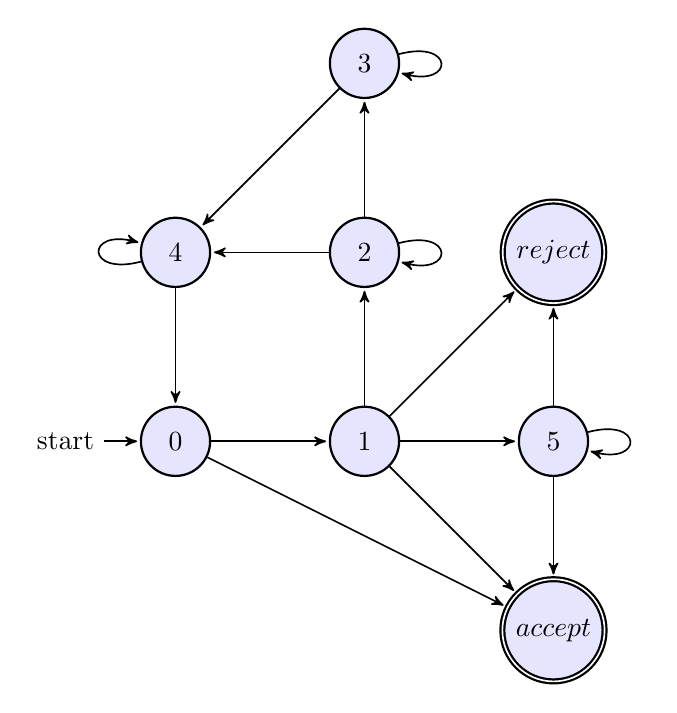
\begin{tikzpicture}[->,>=stealth',shorten >=1pt,auto,node distance=2.4cm,on grid,semithick, every state/.style={fill=blue!10,thick}]
\node[initial,state] 	 (0)              {$0$};
\node[state]        	 (1) [right of=0] {$1$};
\node[state]        	 (5) [right of=1] {$5$};
\node[state]        	 (4) [above of=0] {$4$};
\node[state]        	 (2) [above of=1] {$2$};
\node[state]        	 (3) [above of=2] {$3$};
\node[state,accepting]   (r) [above of=5] {$reject$};
\node[state,accepting]	 (a) [below of=5] {$accept$};

\path[->] 
	(0) edge [below]        node {$  $} (1)
	(0) edge [above]        node {$  $} (a)        
    (1) edge [below]   		node {$  $} (2)
	(1) edge [below]        node {$  $} (5)
    (1) edge [below]   		node {$  $} (r)
    (1) edge [below]   		node {$  $} (a)    
	(2) edge [loop right] 		node {$  $} (2)
	(2) edge [below] 		node {$  $} (3)  
    (2) edge [below] 		node {$  $} (4)  
    (3) edge [loop right] 		node {$  $} (3)  
    (3) edge [below] 		node {$  $} (4)  
    (4) edge [loop left] 		node {$  $} (4)  
    (4) edge [below] 		node {$  $} (0)  
    (5) edge [below] 		node {$  $} (r)
    (5) edge [loop right] 		node {$  $} (5)
    (5) edge [below] 		node {$  $} (a)


    
;    
\end{tikzpicture}\\

% Question 5
5.\\
pseudo-code : 
Assume input string locate in tape 1 and tape 2 is empty.\\
set pointer1 = the end of tape 1\\
set pointer2 = the beginning of tape 2\\
while current pointer location is not the head of tape 1\\
\{\\
    copy the character which pointer1 point at to the location where pointer2 is\\
    pointer1 --\\
    pointer2 ++\\
\}\\
set pointer2 = the beginning of tape 2\\
compare the character of each position in two tapes\\

graph:\\
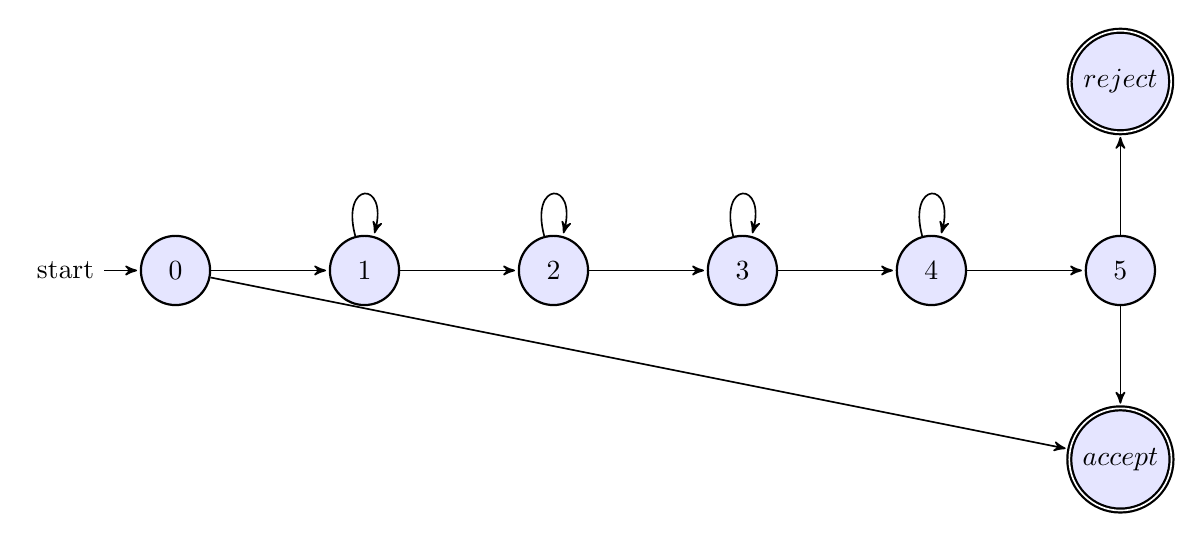
\begin{tikzpicture}[->,>=stealth',shorten >=1pt,auto,node distance=2.4cm,on grid,semithick, every state/.style={fill=blue!10,thick}]
\node[initial,state] 	 (0)              {$0$};
\node[state]        	 (1) [right of=0] {$1$};
\node[state]        	 (2) [right of=1] {$2$};
\node[state]        	 (3) [right of=2] {$3$};
\node[state]        	 (4) [right of=3] {$4$};
\node[state]        	 (5) [right of=4] {$5$};
\node[state,accepting]   (r) [above of=5] {$reject$};
\node[state,accepting]	 (a) [below of=5] {$accept$};

\path[->] 
	(0) edge [below]        node {$  $} (1)
    (0) edge [below]        node {$  $} (a)
    (1) edge [below]   		node {$  $} (2)
    (1) edge [loop above]   		node {$  $} (1)
	(2) edge [loop above] 		node {$  $} (2)
	(2) edge [below] 		node {$  $} (3)  
    (3) edge [loop above] 		node {$  $} (3)  
    (3) edge [below] 		node {$  $} (4)  
    (4) edge [loop above] 		node {$  $} (4)  
    (4) edge [below] 		node {$  $} (5)  
    (5) edge [below] 		node {$  $} (r)
    (5) edge [below] 		node {$  $} (a)

;    
\end{tikzpicture}\\
state explanation(4 processes):\\
0:start\\
1:move pointer1 to the right end of tape1\\
2:copy character from tape1 to tape2 in reverse order\\
3:move pointer2 to the left end of tape2\\
4:compare each character\\

analysis:\\
In the process 1~4 described above, there are n steps. So totally there are 4n steps.\\
O(4n) = O(n)\\

\end{document}